\documentclass[12pt]{article}
%%%%%%%%%%%%%%%%%%%%%%%%%%%%%%%%%%%%%%%%%%%
\usepackage{graphicx}
\usepackage{epsfig}
\usepackage{subfig}
\usepackage{amsmath}
\usepackage{amssymb}
\usepackage{geometry}
\geometry{
	a4paper,
	total={170mm,257mm},
	left=20mm,
	top=20mm,
}
\usepackage{xcolor}
% For correct labelling
%(...)
\usepackage{hyperref}
%%%%%%%%%%%%%%%%%%%%%%%%%%%%%%%%%%%%%%%%%%%

\begin{document}
	
\title{Gaussian Processes for Higgs inclusive}
\author{Jes\'us Urtasun Elizari}
\date{Milan, April 2020}
\maketitle


\newpage
\section{Introduction}
The main goal of this project is to develop an approximate expression to the Higgs inclusive cross section in gluon fusion up to N3LO. For this purpose we develop a Gaussian Process (GP) regressor, a machine learning model that performs interpolation assuming Gaussian distributed input data, and optimizes the so-called covariance functions, or also \textit{kernels}, by training on the asymptotic expressions.\\

After testing a simple version of this gaussian regression, also known as \textit{Kringing}, in the $p_{\perp}$ distribution at leading order in $p_{\perp}$, we aim to improve the performance given the deeper knowledge and various physical constrains that are available in the inclusive case. The roadmap that we follow is shown below.\\

\begin{enumerate}
	\item Generate the NLO, NNLO, N3LO coefficient functions using the numerical implementation done in \href{https://www.ge.infn.it/~bonvini/higgs/}{ggHiggs} code by Marco Bonvini.
	\item Implement the analytic expressions of the asymptotics at the different perturbative orders from \href{https://arxiv.org/abs/1303.3590}{1303.3590}. They will be used as training data as we will explain later in section 4.
	\item Build the Gaussian Process regressor.
	\item Hyperoptimize the Gaussian Process regressor.
\end{enumerate}

The last step is indeed were we aim to obtain the best performance. By performing hyper optimization, or \textit{hyperopt} on the kernels and internal parameters of the gaussian regressor, we scan the whole parameter space to find the best model for making predictions in our particular process. That way the performance will be versatile enough to be extended not only to different perturbative orders in our inclusive case, but also for making predictions in other processes as $p_{\perp}$ distribution in a straightforward way.

\section{Higgs inclusive in gluon fusion}

Our starting point will be to consider the general expression of the inclusive cross section written in terms of the PDFs and the partonic cross section:
\begin{equation}
	\sigma(\tau, m_{H}^{2}) = \tau \sum_{i,j} \int_{\tau}^{1} \; \frac{dz}{z} \;
	\mathcal{L}_{ij} \bigg(\frac{\tau}{z}, \mu_{R}^{2} \bigg) \frac{1}{z} \hat{\sigma}_{ij} \Bigg(z, m_{H}^{2}, \alpha_{s}(\mu_{R}^{2}), \frac{m_{H}^{2}}{\mu_{F}^{2}},  \frac{m_{H}^{2}}{\mu_{R}^{2}} \Bigg), \quad \tau = \frac{m_{H}^{2}}{s}
\end{equation}

being $\mathcal{L}_{ij}(z, \mu^{2})$ the parton luminosity tensors
\begin{equation}
	\mathcal{L}_{ij} (z, \mu^{2}) = \int_{z}^{1} \frac{dx}{x} f_{i}\bigg( \frac{z}{x}, \mu^{2} \bigg) f_{j}(x, \mu^{2})
\end{equation}

Write the cross section in terms of the so called coefficient functions $C_{ij}$
\begin{equation}
	\hat{\sigma}_{ij}\Bigg(z, m_{H}^{2}, \alpha_{s}(\mu_{R}^{2}), \frac{m_{H}^{2}}{\mu_{F}^{2}}, \frac{m_{H}^{2}}{\mu_{R}^{2}} \Bigg) = z \; \sigma_{0} \big(m_{H}^{2}, \alpha_s(\mu_{R}^{2}) \big) \; C_{ij} \Bigg(z, \alpha_{s},  \frac{m_{H}^{2}}{\mu_{F}^{2}}, \frac{m_{H}^{2}}{\mu_{R}^{2}} \Bigg)
\end{equation}

For our further purposes we will work in Mellin space, therefore the function to approximate can be written as follows showing explicitly the powers of $\ln N$, whose behavior is already well known from both small $N$ and large $N$ (soft) resummation.
\begin{equation}
	C_{\textrm{res}}(N, \alpha_{s}) = g_{0}(\alpha_{s}) \Bigg[\frac{1}{\alpha_{s}} g_{1}(\alpha_{s} \ln N) + g_{2}(\alpha_{s} \ln N) + \alpha_{s} g_{3} (\alpha_{s} \ln N) + ...\Bigg]
	\label{resummed}
\end{equation}
with
\begin{equation}
	g_{0}(\alpha_{s}) = 1 + \alpha_{s}g_{0, 1} + \alpha_{s}^{2} g_{0, 2} + \mathcal{O}(\alpha_{s}^{3})
\end{equation}

As explained in section 2 of \href{https://arxiv.org/abs/1303.3590}{1303.3590}, we can use an approximate expression as if we knew the $N$ space resummed coefficient function. Then we could extract from eq. \eqref{resummed} the $\mathcal{O}(\alpha_{s})$ coefficient $C^{(1)}$ as follows
\begin{align}
		C^{(1)}(z) &= 4 A_{g}(z) \mathcal{D}_{1}(z) + d \delta(1 - z) - 2 A_{g}(z)\frac{\ln z}{1-z} + R_{gg}(z), \\
		\mathcal{D}_{k}(x) &\equiv \Bigg( \frac{\ln^{k}(1 - x)}{1 - x} \Bigg)_{+},\\
		A_{g}(z) &= \frac{C_{A}}{\pi} \frac{1 - 2 z + 3 z^{2} - 2 z^{3} + z^{4}}{z}.
\end{align}

The behavior at small $N$ is dominated by the $R_{gg}$ function, which has a complicated structure, and therefore the way we obtain $C^{(n)}(N)$ for higher perturbative orders in N space is by using the numerical implementation performed with \href{https://www.ge.infn.it/~bonvini/higgs/}{ggHiggs} code by Marco Bonvini.
\begin{figure}
	\center
	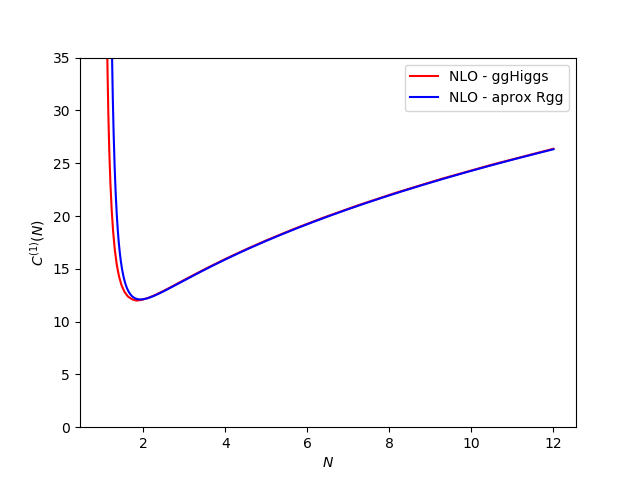
\includegraphics[width = 10cm]{plots/data/check_ggHiggs.png}
	\caption{Comparison between our mathematica implementation of $C^{(1)}(N)$, using the approximate form of $R_{gg}$ in the point-like limit, and ggHiggs, which numerically implements the exact expression. As expected, the deviation starts at small $N$, where the $R_{gg}$ function dominates the behavior.}
	\label{fig:check_data}
\end{figure}

As a warm up exercise we Mellin transform the coefficient function shown above and compare it with the implementation in Bonvini's code. As expected, as long as we increase $N$ and the behavior stops being dominated by $R_{gg}$, both curves show excellent numerical agreement.\\

\section{Asymptotics}

As mentioned before, the asymptotics are computed by following \href{https://arxiv.org/abs/1303.3590}{1303.3590}. Further discussions concerning the N3LO computation can be found in the updated version \href{https://arxiv.org/abs/1404.3204}{1404.3204} We will devote a section below to explain the way the Python implementation was carried out, trying to make it look as clear and user-friendly as possible, since the amount of long algebraic expressions could make non-trivial to follow the calculation for someone not experienced enough with notation.

\subsection{Small $N$}
The leading small $N$ singularities have been determined to all orders in $\alpha_{s}$, for both $m_{t} \rightarrow \infty$ and finite $m_{t}$. Here we just show the result computed at \href{https://arxiv.org/abs/1303.3590}{1303.3590}. By combining the expansion terms of the anomalous dimension $\gamma^{+}$
\begin{align}
	\gamma^{(0)} &= \frac{e_{0, -1}}{N - 1} + e_{00} + \mathcal{O}(N - 1) \\
	\gamma^{(1)} &= \frac{e_{1, -2}}{(N - 1)^{2}} + \frac{e_{1, -1}}{N - 1} + \mathcal{O}(1) \\
	\gamma^{(2)} &= \frac{e_{2, -3}}{(N - 1)^{2}} + \frac{e_{2, -2}}{N - 1} + \mathcal{O}(N - 1)^{-1}
\end{align}
where the coefficients $e_{i, j}$ are constants depending on the $C_{A}$, $C_{F}$ color factors and the number of flavors $n_{f}$, all listed in the appendix. The small $N$ approximation to the coefficient function is obtained as

\begin{figure}
	\centering
	\subfloat[NLO]{{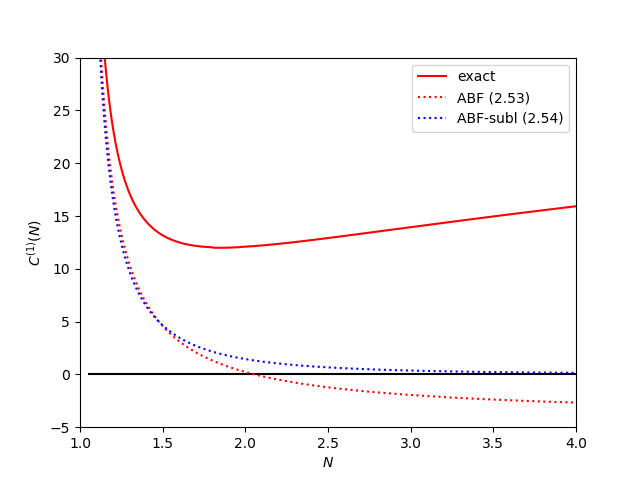
\includegraphics[width = 8cm]{plots/data/nlo_small_n.png}}}
	\qquad
	\subfloat[NNLO]{{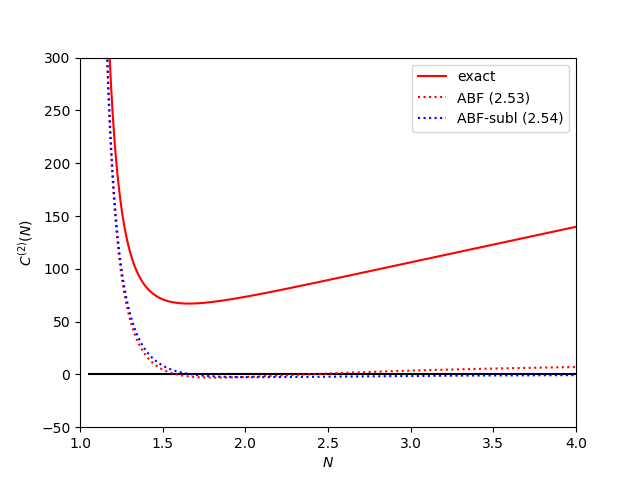
\includegraphics[width = 8cm]{plots/data/nnlo_small_n.png} }}
	\caption{Different asymptotic expressions at small $N$ together with the exact computation of the Higgs cross section at NLO (left) and NNLO (right), reproducing figure 2 of \href{https://arxiv.org/abs/1303.3590}{1303.3590} with our Python implementation of the asymptotics.}.
	\label{small_n_asymptotics}
\end{figure}

\begin{align}
	C_{\textrm{ABF}} (N, \alpha_{s} ) &= \sum_{n = 1}^{\infty} \alpha_{s}^{n} C_{\textrm{ABF}}^{(n)}(N) \\
	& = \sum_{i_{1}, i_{2} \geq 0} c_{i_{1}, i_{2}} \bigg[ \gamma^{+i_{1}} \bigg] \bigg[ \gamma^{+i_{2}} \bigg] - 1\\
	&= \alpha_{s} 2 c_{1, 0} \gamma^{(0)} \\ \nonumber
	& \hspace{0.5cm} + \alpha_{s}^{2} \Bigg[(2 c_{2, 0} + c_{1, 1}) \gamma^{(0)^{2}} - 2 c_{2, 0} \beta_{0} \gamma^{(0)} + 2 c_{1, 0} \gamma^{(1)} \Bigg] \\
	& \hspace{0.5cm} + \alpha_{s}^{3} \Bigg[(c_{3, 0} + c_{2, 1})2\gamma^{(0)^{3}} - 3 (c_{3, 0} + c_{2, 1}) 2 \beta_{0} \gamma^{(0)^{2}} + 4c_{3, 0}\beta_{0}^{2}\gamma^{(0)} \\ \nonumber
	& \hspace{2.0cm} + (2c_{2, 0} + c_{1, 1})2\gamma^{(0)}\gamma^{(1)} - 4c_{2, 0}\beta_{0}\gamma^{(1)} + 2c_{1, 0}\gamma^{(2)} \Bigg] \\ \nonumber
	& \hspace{0.5cm} + \mathcal{O}(\alpha_{s}^{4})
\end{align}
We can also use an improved, or \textit{subleading} version, built by subtracting the expression above in such a way that it keeps the small $N$ behavior but that ensures vanishing behavior also at $N \rightarrow \infty$.
\begin{align}
C_{\textrm{ABF-subl}}^{(n)}(N) = C_{\textrm{ABF}}^{(n)}(N) - 2 C_{\textrm{ABF}}^{(n)}(N + 1) + C_{\textrm{ABF}}^{(n)}(N + 2)
\end{align}
The subtraction only introduces subleading $N = 0$ and $N = -1$ singularities. Different possible choices are perfectly allowed on how to perform the subtraction.

\subsection{Large $N$}
In the large N (soft) approximation we find powers of  $\ln N$ which are just the large $N$ approximation of the digamma function $\psi_{0}(N)$  appearing in fix order computations. This part of the coefficient function is written as combinations of the $\mathcal{D}_{k}(N)$, $\hat{\mathcal{D}}_{k}(N)$, $\mathcal{D}^{log}_{k}(N)$ distributions, which involve the polygamma functions as defined in Appendix (A.6) of \href{https://arxiv.org/abs/1303.3590}{1303.3590}. We show here their definition in direct $x$ space
\begin{align}
	\mathcal{D}_{k}(x) &\equiv \Bigg( \frac{\ln^{k}(1 - x)}{1 - x} \Bigg)_{+} ,\\
	\mathcal{D}_{k}^{log}(x) &\equiv \Bigg( \frac{\ln^{k}\ln\frac{1}{x}}{\ln\frac{1}{x}} \Bigg)_{+}, \\
	\hat{\mathcal{D}}_{k}(x) &\equiv \mathcal{D}_{k}(x) + \Bigg[ \frac{\ln^{k}\ln\frac{1 - x}{\sqrt{x}}}{1 - x} - \frac{\ln^{k}(1 - x)}{1 - x} \Bigg],
\end{align}

And their Mellin expressions as defined in appendix A of \href{https://arxiv.org/abs/1303.3590}{1303.3590}, or equivalently from appendix B of \href{https://arxiv.org/pdf/1212.0480.pdf}{1212.0480}. By combining them we obtain the $S(N)$ combinations that will be used to write down the soft approximations. From (2.36)
\begin{align}
	C_{\textrm{soft1}}(N) &= \bar{g}_{0}(\alpha_{s}) \exp \sum_{n = 1}^{\infty} \alpha_{s}^{n} \sum_{k = 0}^{n} b_{n, k} \; \hat{\mathcal{D}}_{k}(N + 1) \\
	C_{\textrm{soft2}}(N) &= \bar{g}_{0}(\alpha_{s}) \exp \sum_{n = 1}^{\infty} \alpha_{s}^{n} \sum_{k = 0}^{n} b_{n, k} \; \bigg[ 2\hat{\mathcal{D}}_{k}(N) - 3\hat{\mathcal{D}}_{k}(N + 1) + 2\hat{\mathcal{D}}_{k}(N + 2) \bigg]
\end{align}
and (2.39) 
\begin{align}
	C_{\textrm{soft}}(N, \alpha_{s}) &= \bar{g}_{0}(\alpha_{s}) \exp \sum_{n = 1}^{\infty} \alpha_{s}^{n} S_{n}(N)
\end{align}
we identify the $S_{n}$(N) expressions that lead to the soft approximations at the different perturbative orders. Again, a detailed description of the way all asymptotic expressions are obtained from the paper, leading to reproducing every figure on it and taking full control of the input data for our GP, is explained below. One arrives to build 

\begin{figure}
	\centering
	\subfloat[NLO]{{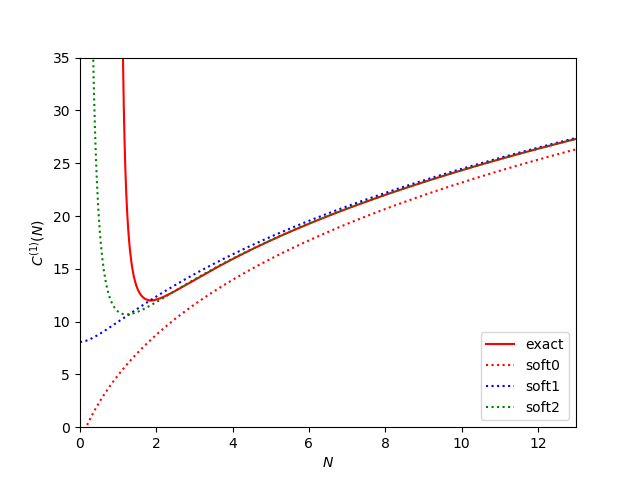
\includegraphics[width = 8cm]{plots/data/nlo_large_n.png}}}
	\qquad
	\subfloat[NNLO]{{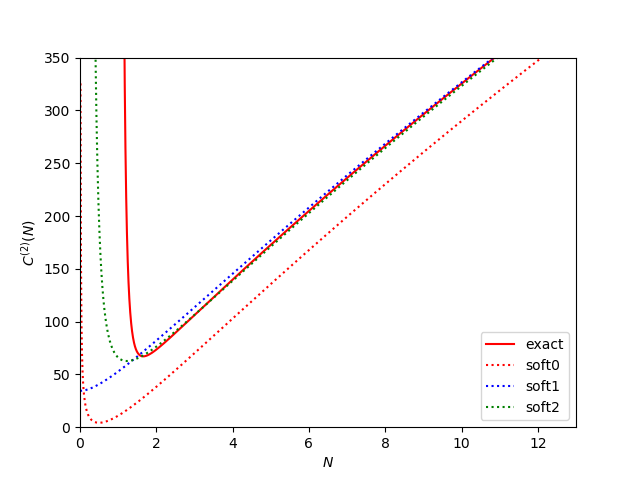
\includegraphics[width = 8cm]{plots/data/nnlo_large_n.png} }}
	\caption{Different asymptotic expressions at large $N$ together with the exact computation of the Higgs cross section at NLO (left) and NNLO (right), reproducing figure 1 of \href{https://arxiv.org/abs/1303.3590}{1303.3590} with our Python implementation of the asymptotics.}
	\label{large_n_asymptotics}
\end{figure}

\begin{align}
	C_{\textrm{soft}}^{(1)} &= S_{1}(N) + \bar{g}_{0, 1} \\
	C_{\textrm{soft}}^{(2)} &= \frac{1}{2}S_{1}^{2}(N) + S_{2}(N) + \bar{g}_{0, 1}S_{1}(N) + \bar{g}_{0, 2} \\
	C_{\textrm{soft}}^{(3)} &= \frac{1}{6}S_{1}^{3}(N) + S_{1}(N)S_{2}(N) + S_{3}(N) + \bar{g}_{0, 1}\bigg( \frac{1}{2}S_{1}^{2}(N) + S_{2}(N) \bigg) + \bar{g}_{0, 2}S_{1}(N) + \bar{g}_{0, 3}.
\end{align}

We choose the asymptotic expression labeled as $\textrm{soft}_{1}$ as the large $N$ asymptotics as training data in that region. At small $N$, we find no remarkable difference when changing from the $C_{ABF}$ to its subleading version.

\subsection{N3LO discussion}
\begin{enumerate}
	\item Asymptotics still to be fully implemented for N3LO. Check updated version \href{https://arxiv.org/abs/1404.3204}{1404.3204}. 
	\item Reproduce figures 4 and 5 of \href{https://arxiv.org/abs/1303.3590}{1303.3590} together with figure 4
	\href{https://arxiv.org/pdf/1805.08785.pdf}{1805.08785}
	\item As a next step, try also to interpolate from previous orders given the convergence shown in figure 8 of \href{https://arxiv.org/abs/1303.3590}{1303.3590} rather from the asymptotics.	
\end{enumerate}

\newpage

\section{Gaussian Processes for inclusive observables}
Now we are ready to start training our machine learning gaussian regressor. This kind of interpolation begins by assuming that the function to guess is sampled from a Gaussian distribution $f(x) \sim N(\mu, K(\theta, x, x'))$, where $K(\theta, x, x')$ is the covariance matrix between all possible points $x, x'$ given a set of parameters $\theta$ (such as the length scale of the kernel, periodicity if any, or more specific parameters concerning the definition of the kernels). The way we will apply the interpolation goes as follows
\begin{enumerate}
	\item Take the asymptotics computed at \href{https://github.com/N3PDF/crystalball/blob/jesus_gp/asymptotics/check_n3lo_data.py}{{\color{blue}check\_n3lo\_data.py}} by following \href{https://arxiv.org/abs/1303.3590}{1303.3590} as input (training) data.
	\item Assume the points $x$ are sampled from a Gaussian distribution $f(x) \sim N(\mu, K(\Theta, x, x'))$.
	\item Train $\Theta$ by minimizing a $\chi^{2}(f(x)|\Theta, x)$ to guess the underlying law.
	\item Use the Mellin-space exact coefficient functions computed by \href{https://www.ge.infn.it/~bonvini/higgs/}{ggHiggs} as true values for testing and validation.
\end{enumerate}

\subsection{Implement asymptotics}
As said before, we devote a section to provide a detailed description of the way the Python implementation of the asymptotics was carried out, and its comparison with the exact coefficient functions, trying to make it look as accessible and user-friendly as possible towards other possible applications. On the  \href{https://github.com/N3PDF/crystalball/tree/jesus_gp/asymptotics}{asymptotics} folder of the N3PDF repository they are organize as follows. 

\begin{enumerate}
	\item The main file \href{https://github.com/N3PDF/crystalball/blob/jesus_gp/asymptotics/check_n3lo_data.py}{{\color{blue}check\_n3lo\_data.py}} reproduces the different figures in the paper by first loading the exact curves from ggHiggs and then calling the asymptotic expressions.
	\item The \href{https://github.com/N3PDF/crystalball/blob/jesus_gp/asymptotics/contributions_small_n.py}{{\color{blue}contributions\_small\_n.py}} file contains the expansions of the anomalous dimension $\gamma^{(i)}$ together with the small $N$ asymptotics labeled as ABF and ABF-subl, following the notation from the paper, up to N3LO.
	\item The \href{https://github.com/N3PDF/crystalball/blob/jesus_gp/asymptotics/contributions_large_n.py}{{\color{blue}contributions\_large\_n.py}} file holds for the explicit expressions for the $\mathcal{D}_{k}(N)$, $\mathcal{D}^{log}_{k}(N)$ and $\hat{\mathcal{D}}_{k}(N)$ distributions, their combinations $S(N)$ and the large $N$ asymptotics labeled as soft-0, soft-1, soft-2, following the notation from the paper, up to N3LO.
	\item File \href{https://github.com/N3PDF/crystalball/blob/jesus_gp/asymptotics/check_data.py}{{\color{blue}check\_data.py}} computes the comparison shown in figure \ref{fig:check_data} together with some old checks of the first implementations of the asymptotics.
\end{enumerate}


To begin with we set some ground values for the point at we stop the training asymptotics, defining the interpolation region. They can be changed, together with the number of points used for training, as a next step towards a more fine tuned performance.
\begin{figure}
	\centering
	{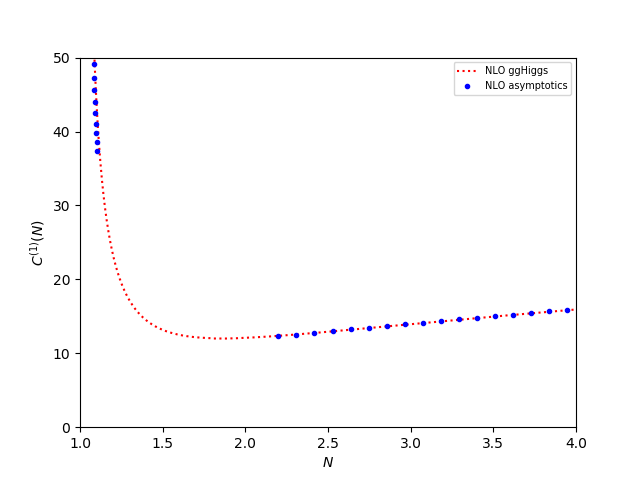
\includegraphics[width = 8cm]{plots/nlo_asymptotics.png}}
	\qquad
	{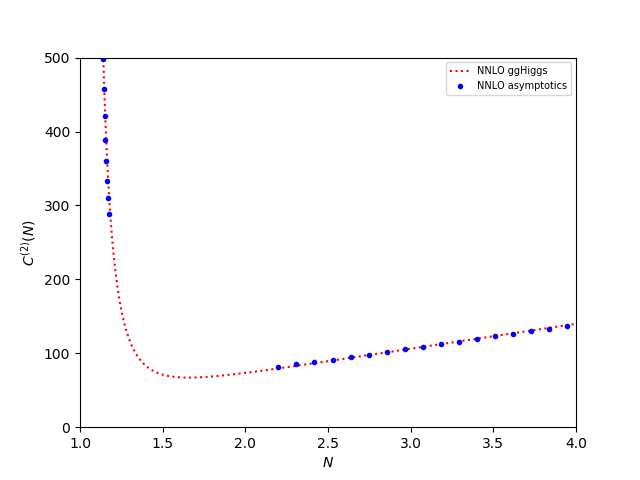
\includegraphics[width = 8cm]{plots/nnlo_asymptotics.png}}
	\caption{Representation of the asymptotics (training data) and exact inclusive coefficient function (testing and validation) at NLO (left) and NNLO (right) as a function of N.}
	\label{asymptotics_gp}
\end{figure}

\newpage

\subsection{Covariance functions}
The key object we aim to train for performing an optimal interpolation is the so called \textit{kernel}, or \textit{covariance function}, also known as covariance matrix.
The different kernels tried for our process are the following, \href{https://scikit-learn.org/stable/modules/classes.html#module-sklearn.gaussian_process}{scikit-learn-kernels}

\subsubsection{Constant kernel}
The Constant kernel is the simplest case. It can be used as part of a product kernel where it scales the magnitude of the other kernel or as part of as part of a sum kernel, where it modifies the mean of the gaussian process. It depends on a parameter $C$ and it is defined as:
\begin{equation}
k(x_{i}, x_{j}) = C \; \forall \; x_{i} x_{j}
\end{equation}

\subsubsection{RBF}
The Radial Basis Function (RFB) kernel is also known as the “squared exponential” kernel. It is parameterized by a length-scale parameter $l > 0$ , which can either be a scalar (isotropic variant of the kernel) or a vector with the same number of dimensions as the inputs  (anisotropic variant). For our case lets consider the isotropic variant, where the kernel is given by
\begin{equation}
k(x_{i}, x_{j}) = \exp \bigg( -\frac{1}{2} d\big(x_{i}/l, x_{j}/l\big)^{2} \bigg)
\end{equation}

This kernel is infinitely differentiable, which implies that GPs with this kernel as covariance function have mean square derivatives of all orders, and are thus very smooth.

\subsubsection{Matern}
The Matern kernel is a stationary kernel and a generalization of the RBF kernel. It has an additional parameter  which controls the smoothness of the resulting function. It is parameterized by a length-scale parameter , which can either be a scalar (isotropic variant of the kernel) or a vector with the same number of dimensions as the inputs  (anisotropic variant). The kernel is given by

\begin{equation}
k(x_{i}, x_{j}) = \sigma^{2} \frac{1}{\Gamma(\nu)2^{\nu - 1}}
\Bigg(\gamma \sqrt{2\nu} d\big(x_{i}/l, x_{j}/l\big)\Bigg)^{\nu} K_{\nu} \Bigg(\gamma \sqrt{2\nu} d\big(x_{i}/l, x_{j}/l\big)\Bigg)
\end{equation}

when $\nu \rightarrow \infty$, the Matern kernel tends to the RBF. Other popular choices are also $\nu = 3/2$ and $\nu = 5/2$, leading to a one-time and two-times differentiable kernel, respectively (add documentation...)

\subsubsection{Rational Quadratic} 
The Rational Quadratic kernel can be seen as a scale mixture, or infinite sum, of RBF kernels with different characteristic length-scales. It is parameterized by a length-scale parameter $l > 0$ and a scale mixture parameter $\alpha > 0$. Only the isotropic variant where $l$ is a scalar is supported at the moment. The kernel is given by:
\begin{equation}
k(x_{i}, x_{j}) = \Bigg( 1 + \frac{d\big(x_{i}, x_{j}\big)}{2\alpha l^{2}} \Bigg)^{-\alpha}
\end{equation}

\subsubsection{Exp-sin}
The ExpSineSquared kernel allows modeling periodic functions. It is parameterized by a length-scale parameter $l > 0$ and a periodicity parameter $p > 0$.
\begin{equation}
k(x_{i}, x_{j}) = \exp \Bigg( -2 \sin(\pi/p \cdot d\big(x_{i}, x_{j}\big) ) /l )^{2} \Bigg)
\end{equation}
This is an example of the kind of kernel we do not expect to perform in an optimal way to our problem, given the asymmetry of the function to interpolate, and indeed it is shown to be a bad choice in figure (Add figure example ...)

\subsubsection{Dot product}
The Dot Product kernel can be obtained from linear regression by putting $N(0, 1)$ priors on the coefficients of $x_{d}(d = 1, ..., D)$ and a prior $N(0, \sigma_{0^{2}})$ on the bias. The Dot Product kernel is invariant to a rotation of the coordinates about the origin, but not translations. It is parameterized by a parameter $\sigma_{0^{2}}$. For $\sigma_{0^{2}} = 0$, the kernel is called the homogeneous linear kernel, otherwise it is inhomogeneous. The kernel is given by
\begin{equation}
k(x_{i}, x_{j}) = \sigma_{0}^{2} + x_{i} \cdot x_{j}
\end{equation}
This kernel is also shown to be far from a good choice, as models involving it lead to extremely high $\chi^{2}$ after training.

\newpage

\subsection{Hyperoptimization}
After running over different kernels we already saw that when applying the gaussian regression for the $p_{\perp}$ that different choices of the covariance functions lead to very different performance, and we already find some of them performing good interpolation, trained by comparing with data using a $\chi^{2}$ estimator. As said, over all available kernels and using their default parameters listed in \href{https://scikit-learn.org/stable/modules/classes.html#module-sklearn.gaussian_process}{ scikit-learn kernels}, we see that the ones that perform better given the $1 - \chi^{2}$ score used are the Matern, Rational Quadratic, together with linear combinations and products between them all, as shown in figures \ref{nlo_examples} and \ref{nnlo_examples}.

\begin{enumerate}
	\item The \href{https://github.com/N3PDF/crystalball/blob/jesus_gp/HyperGP_inclusive_Nspace.py}{{\color{blue}HyperGP\_inclusive\_Nspace.py}} main file performs the hyperopt and the Gaussian Process regression for the Higgs inclusive cross section.
	\item The
	\href{https://github.com/N3PDF/crystalball/blob/jesus_gp/HyperGP_pt_distribution.py}{{\color{blue}HyperGP\_pt\_distribution.py}} file performs the hyperopt and the Gaussian Process regression for the Higgs $p_{\perp}$ distribution (work in progress).
	\item Both files rely on the \href{https://github.com/N3PDF/crystalball/blob/jesus_gp/HyperGP.py}{{\color{blue}HyperGP.py}} class, which we inherit from the Gaussian Process regressor and manually to manually set the desired parameters, such as the kernels, their internal parameters and the way the score is computed, as training parameters to be optimized.
	\item The \href{https://github.com/N3PDF/crystalball/blob/jesus_gp/summary/nlo_hyperopt.txt}{{\color{blue}nlo\_hyperopt.txt}} stores all parameter dictionaries, together with their scores achieved during they hyperopt process for the NLO search.
	\item The \href{https://github.com/N3PDF/crystalball/blob/jesus_gp/summary/nnlo_hyperopt.txt}{{\color{blue}nnlo\_hyperopt.txt}} stores all parameter dictionaries, together with their scores achieved during they hyperopt process for the NNLO search.
\end{enumerate}

The way the hyperoptimization is implemented is by instancing a  \href{https://scikit-learn.org/stable/modules/generated/sklearn.model_selection.GridSearchCV.html}{Grid Search} to run non only over the list of mentioned kernels, but scan all parameter space to find the best combination for our model. The different combinations to try are given to the model as a dictionary of parameters to tune. One advantage of the Grid Search implementation is that it allows for the activation of a cross validation mechanism, that performs a validation of every model with some subset of the training set. \\

The way to perform the search and selection of the best model is by applying cross validation, selecting a fraction of the training data to compare with the exact coefficient function by computing a score $1 - \chi^{2}$. That way, once a model is chosen to train it has already been tested (validated) by computing a prediction for a discrete number of points and comparing it with the validation set. The definition of the training - validation split can be modified as an argument to the file \href{https://github.com/N3PDF/crystalball/blob/jesus_gp/HyperGP_inclusive_Nspace.py}{{\color{blue}HyperGP\_inclusive\_Nspace.py}}, while the specific way the score is defined is set in the class \href{https://github.com/N3PDF/crystalball/blob/jesus_gp/HyperGP.py}{{\color{blue}HyperGP.py}}. \\

Then the model chosen as the best one is trained performing the usual $\chi^{2}$ minimization. Results so far are shown in tables \ref{table:hyperopt_NLO}, \ref{table:hyperopt_NNLO}, together with examples of the performance for different parameter sets in figures \ref{nlo_examples} and \ref{nnlo_examples}.

\begin{table}
	\centering
	\vspace{0.5cm}
	\begin{tabular}{|c|c|c|}
		\hline
		Kernel & Best parameter set & $\chi^{2}$ \\
		\hline
		Matern & $l = 0.9, \nu = 0.9$ & 0.28365 \\
		\hline
		Matern & $l = 1.0, \nu = 0.9$ & 0.21115 \\
		\hline
		Matern & $l = 1.3, \nu = 0.9$ & 0.22024 \\
		\hline
	\end{tabular}
	\caption{Example of the best parameter sets found for interpolation at NLO with with $N$ range (1.075, 2.1), together with the $\chi^{2}$ achieved after training. As shown, Matern is the best kernel found so far.}
	\label{table:hyperopt_NLO} 
\end{table}

\begin{table}
	\centering
	\vspace{0.5cm}
	\begin{tabular}{|c|c|c|}
		\hline
		Kernel & Best parameter set & $\chi^{2}$ \\
		\hline
		Matern & $l = 0.8, \nu = 1.0$ & 0.02413 \\
		\hline
		Matern & $l = 0.9, \nu = 1.0$ & 0.02069 \\
		\hline
		Sum2 & $l = 1.3, \nu = 0.9,\alpha = 0.8$ & 0.41660 \\
		\hline
	\end{tabular}
	\caption{Example of the best parameter sets found for interpolation at NNLO with with $N$ range (1.075, 2.1), together with the $\chi^{2}$ achieved after training. As shown, Matern and Sum2, consisting in the sum of a Matern and a Rational Quadratic kernel, are the best choices found so far.}
	\label{table:hyperopt_NNLO}
\end{table}

\newpage

\begin{figure}
	\centering
	
	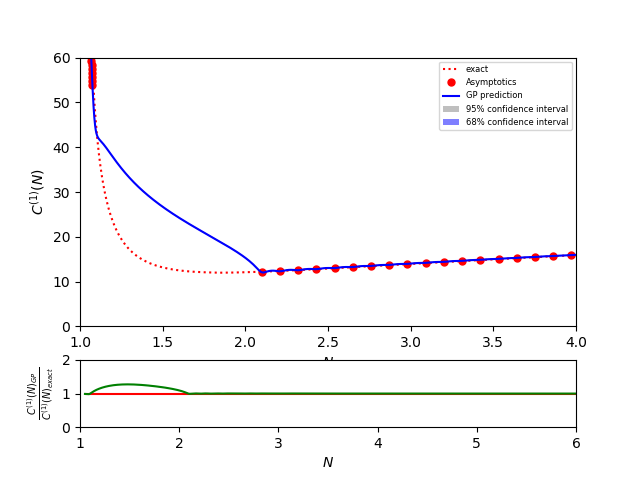
\includegraphics[width=0.6\textwidth]{plots/nlo_test_rquad.png}
	
	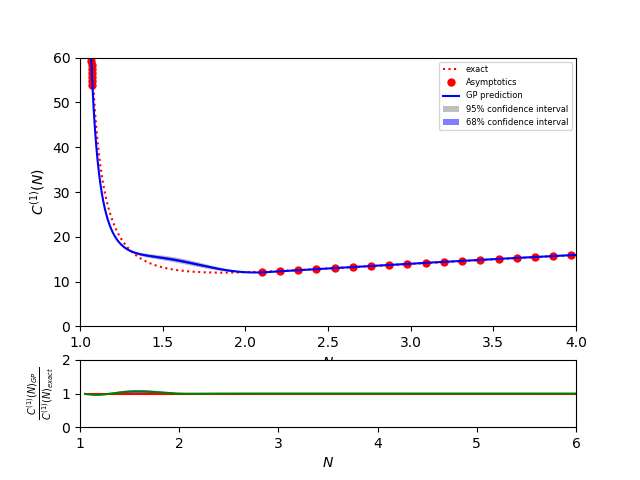
\includegraphics[width=0.6\textwidth]{plots/nlo_test_matern.png}
	
	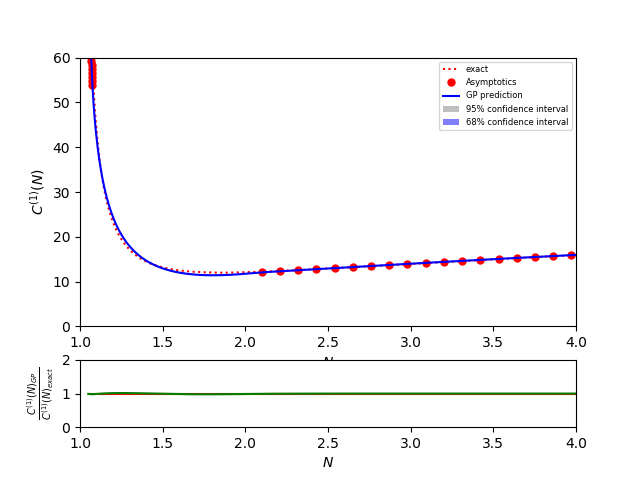
\includegraphics[width=0.6\textwidth]{plots/nlo_matern2.png}
	
	\caption{Example of the interpolation performed at NNLO by different parameter sets as a function of $N$. The example below shows the performance done by the parameter set that obtained the best score so far, with values shown in table \ref{table:hyperopt_NLO}.}
	\label{nlo_examples}

\end{figure}

\begin{figure}
	\centering
	
	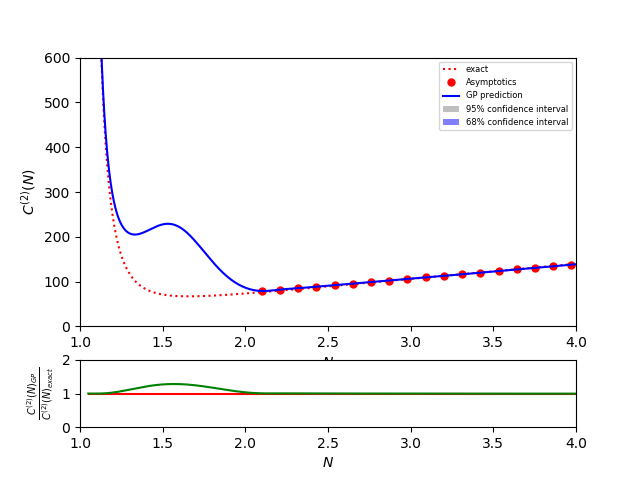
\includegraphics[width=0.6\textwidth]{plots/nnlo_prod2.png}
	
	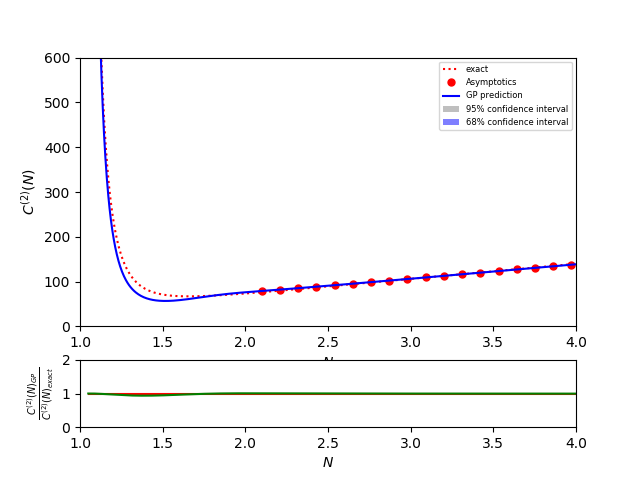
\includegraphics[width=0.6\textwidth]{plots/nnlo_sum2.png}
	
	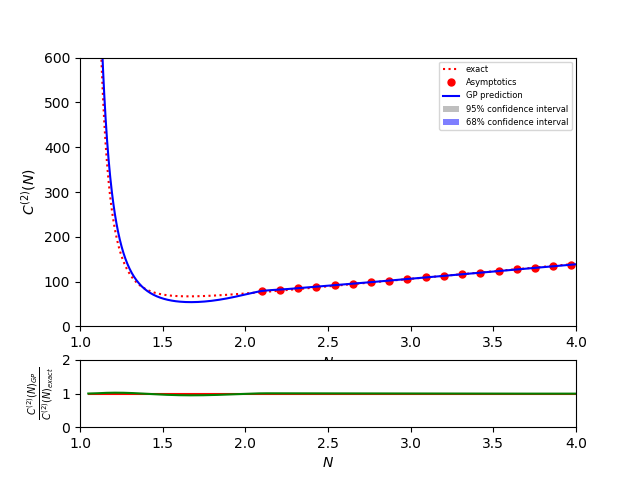
\includegraphics[width=0.6\textwidth]{plots/nnlo_matern.png}
	
	\caption{Example of the interpolation performed at NNLO by different parameter sets as a function of $N$. The example below shows the performance done by the parameter set that obtained the best score so far, with values shown in table \ref{table:hyperopt_NNLO}.}
	\label{nnlo_examples}
	
\end{figure}

\end{document}